\chapter{Relation between Cloud Computing and Docker}

\section{Docker}

\paragraph{\hspace{24pt}}
A docker is an open source enterprise, which can be used to launch any type of application/module as a light- weight container.

\paragraph{\hspace{24pt}}
Due to dockers, there is independence between applications, infrastructure, developers and IT ops. This unlocks their potentials and a model is created for better collaboration and innovation.

\paragraph{\hspace{24pt}}
A docker is simple, agile, secure, portable and also reduces cost.

\section{Relation between Cloud Computing and Docker}

\textbf{Docker with PaaS:} {Dockers are used as fundamental units by various service providers. These include AWS Elastic Beanstalk, OpenShift or Dokku. PaaS provides automation as well as the coding environment. This should be flexible and available on demand. There shouldn’t be any downtime or delay. There has been a shift from virtual machines to docker containers in many IaaS layers.}\\

\textbf{Docker with IaaS:} {Besides coding environment, there is a provision for computing platforms or a virtual server which is completely isolated from the host. It is very easy to setup a docker cluster which may have an installed webserver.}\\

\section{Container}

\paragraph{\hspace{24pt}}
“A container image is a lightweight, stand-alone, executable package of a piece of software that includes everything needed to run it: code, runtime, system tools, system libraries, settings.”

\paragraph{\hspace{24pt}}
It is available for both Windows and Linux based applications. We can call it platform-independent since the “containerized software will always run the same, whatever be the environment.”

\paragraph{\hspace{24pt}}
The containers isolate the software from its environment, This helps in minimizing the conflicts between groups running different software or application on the same infrastructure.

\section{Container Clustering}

\paragraph{\hspace{24pt}}
The job of the container is to turn a number of docker engines into one, single body or entity. This means that the management and launch of containers in multiple systems works as a single body. Container Clustering can be achieved by utilizing the Swarm Manager.

\section{GlusterFS}

\paragraph{\hspace{24pt}}
GlusterFS is a network file system developed by RedHat. It allows the storage of objects and files in cluster of storage servers. It stores the data in a distributed manner. This can be done either by stripping the data or replicating the data or both on multiple storage servers. GlusterFS is a scale-out network-attached file storage system. GlusterFS can be used for various applications such as cloud computing, streaming media services, and content delivery networks. GlusterFS was developed originally by Gluster, Inc. However, Gluster, Inc. was acquired by RedHat in 2011.

\section{Encryption over Cloud Model and its Process using Container}

\subsection{Swarm Manager}

\paragraph{\hspace{24pt}}
The job of a Swarm Manager is to send the plain text(unencrypted) code from the user a node which is running Docker Cryptography Container. Algorithms such as RSA and AES can be used for encryption of the file being uploaded.

\paragraph{\hspace{24pt}}
After encryption, the encrypted data is sent here. SSH protocol is used to handle the transaction of the files.

\paragraph{\hspace{24pt}}
After the transaction, the data is encrypted. However, it needs to be stored such that it is highly available. After the data is encrypted, it is sent back to a Gateway Manager.

\paragraph{\hspace{24pt}}
The data from the Gateway Manager is then sent to another node containing Storage manager(GlusterFS) This storage manager is connected to a new node containing multiple Docker containers. Then the encrypted data is distributed. GlusterFS is used to store the container cluster. By doing this, the encrypted files will be stored on multiple docker containers, thus forming a cluster of storage. This enables us to store data in chunks. This prevents the attacker from gaining the data since even if the node is compromised, the attacker will still have to target the containers. However, each container does not contain all the data as the data was distributed in previous steps. Here, having multiple containers helps.

\paragraph{\hspace{24pt}}
Similarly, we use the same process for decryption. First, the user downloads the required file, then the file is decrypted by the docker image and sent to the swarm manager, and from there the decrypted file is received.

\paragraph{\hspace{24pt}}
The following diagram shows the exact working model of Container Clustering using Dockers for Securing data on Cloud Servers or Storage.

\begin{figure}[htb]
\centering
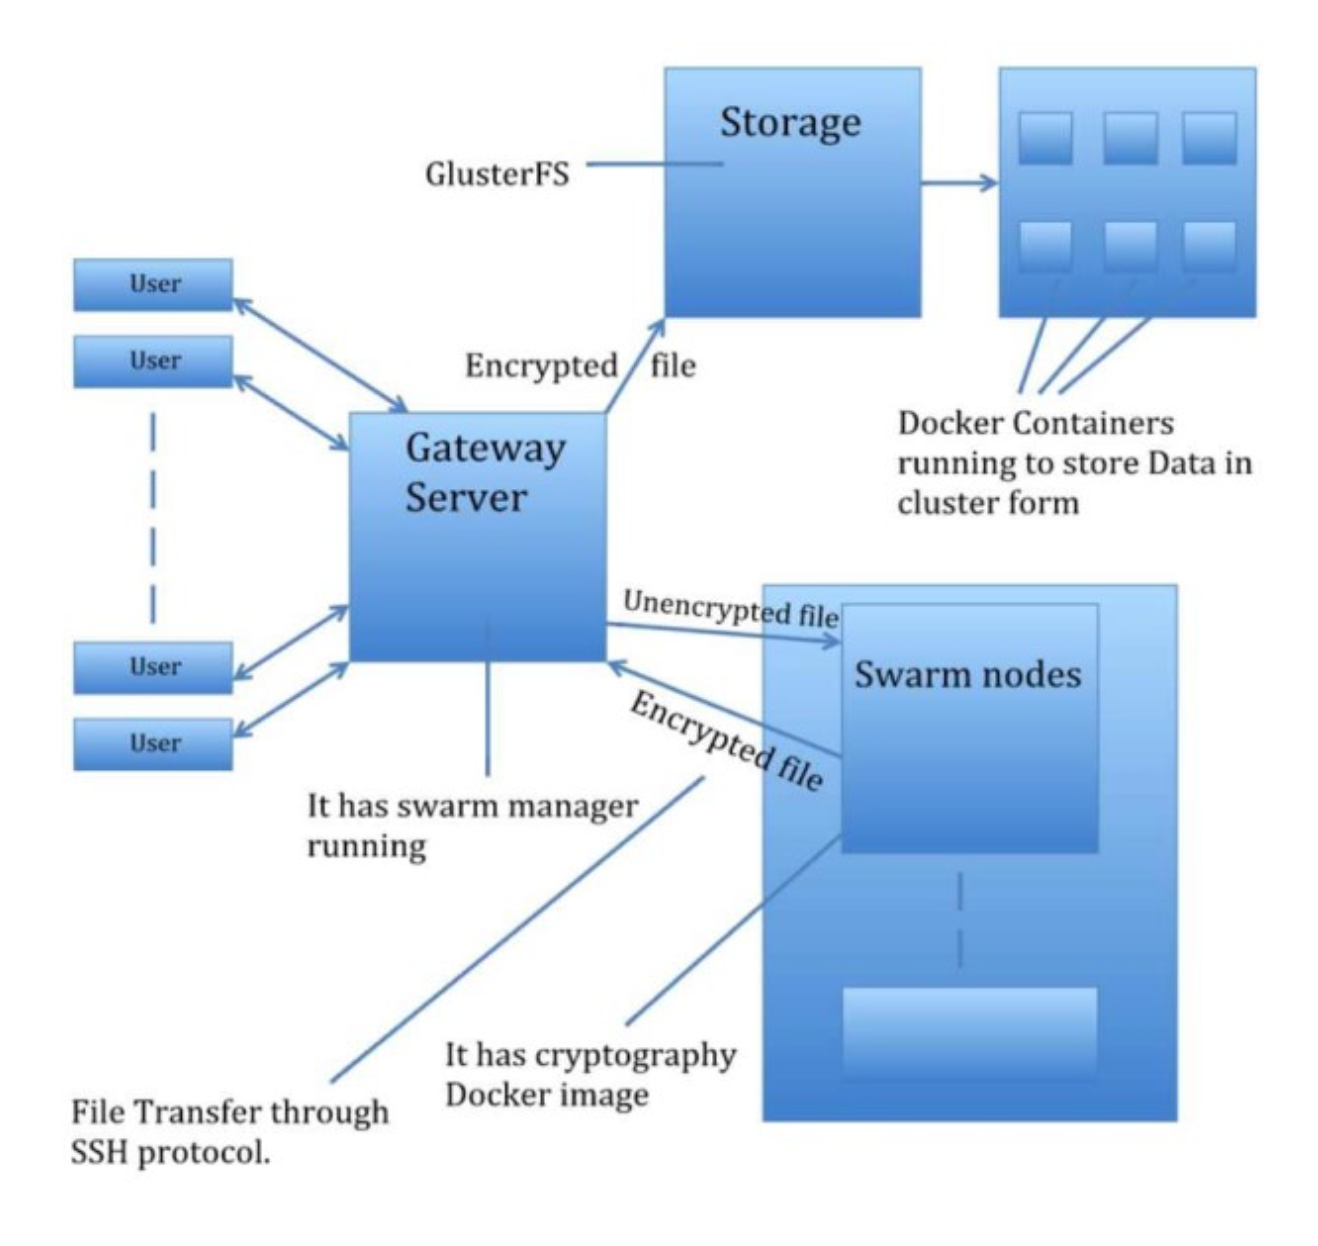
\includegraphics[width=12cm,height=8cm]{5-contents/3-what-is-docker-relation-between-cloud-computing-and-docker/images/container-clustering-docker.png} % e.g. insert ./image for image.png in the working directory, adjust scale as necessary
\caption{Container Clustering Docker}
\label{fig:label} % insert suitable label, this is used to refer to a fig from within the text as shown above
\end{figure}

\begin{figure}[htb]
\centering
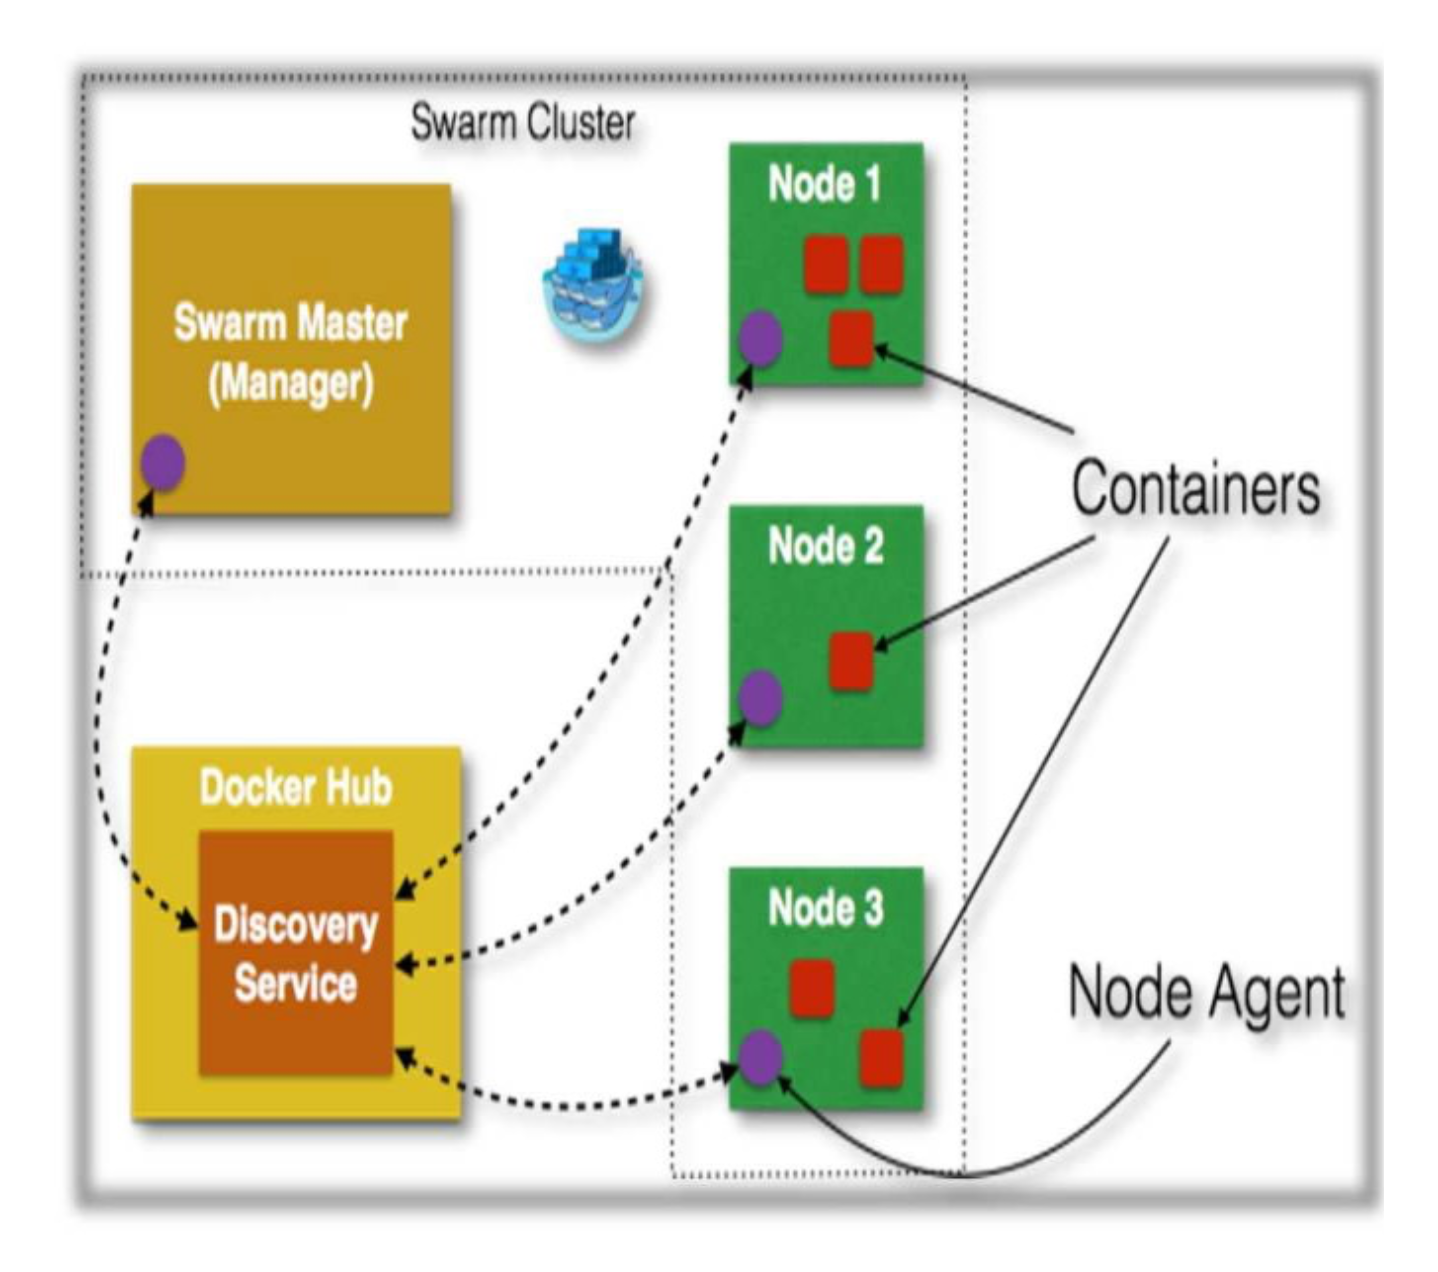
\includegraphics[width=12cm,height=8cm]{5-contents/3-what-is-docker-relation-between-cloud-computing-and-docker/images/docker-swarm-layout.png} % e.g. insert ./image for image.png in the working directory, adjust scale as necessary
\caption{Docker Swarm Layout}
\label{fig:label} % insert suitable label, this is used to refer to a fig from within the text as shown above
\end{figure}